% v2-acmtog-sample.tex, dated March 7 2012
% This is a sample file for ACM Transactions on Graphics
%
% Compilation using 'acmtog.cls' - version 1.2 (March 2012), Aptara Inc.
% (c) 2010 Association for Computing Machinery (ACM)
%
% Questions/Suggestions/Feedback should be addressed to => "acmtexsupport@aptaracorp.com".
% Users can also go through the FAQs available on the journal's submission webpage.
%
% Steps to compile: latex, bibtex, latex latex
%
% For tracking purposes => this is v1.2 - March 2012
\documentclass{acmtog} % V1.2
\usepackage{amsmath,amscd,amsbsy,amssymb,latexsym,url,bm,amsthm}
\usepackage{epsfig,graphicx,subfigure}
\usepackage{enumitem,balance,mathtools}
\usepackage{wrapfig}
\usepackage{subfigure}
\usepackage{mathrsfs, euscript}
\usepackage{hyperref}
\usepackage{listings}
\usepackage{enumerate}
\usepackage{xcolor}
\usepackage{color}
\usepackage[ruled,lined,boxed,linesnumbered]{algorithm2e}
\usepackage[normalem]{ulem}
\useunder{\uline}{\ul}{}
\newtheorem{corollary}[theorem]{Corollary}
\newtheorem{exercise}{Exercise}[section]
\newtheorem*{solution}{Solution}

\begin{document}

\markboth{Recommendation Algorithm}{Collaborative Filtering Algorithm Optimization}

\title{Collaborative Filtering Algorithm Optimization} % title

\author{Hongying Ma {\upshape and} Jiameng Pan
\affil{Shanghai Jiao Tong University}
% NOTE! Affiliations placed here should be for the institution where the
%       BULK of the research was done. If the author has gone to a new
%       institution, before publication, the (above) affiliation should NOT be changed.
%       The authors 'current' address may be given in the "Author's addresses:" block (below).
%       So for example, Mr. Fogarty, the bulk of the research was done at UIUC, and he is
%       currently affiliated with NASA.
}
%\acmVolume{VV}
%\acmNumber{N}
%\acmYear{YYYY}
%\acmMonth{Month}
%\acmArticleNum{XXX}
%\acmdoi{10.1145/XXXXXXX.YYYYYYY}
\acmVolume{28}
\acmNumber{4}
\acmYear{2019}
\acmMonth{September}
\acmArticleNum{106}
\acmdoi{10.1145/1559755.1559763}

\maketitle

\section{Introduction}
Recommender systems typically produce a list of recommendations in one of two ways\cite{jafarkarimi2012naive} – through collaborative filtering or through content-based filtering. Collaborative filtering approaches build a model from a user's past behaviour (items previously purchased or selected and/or numerical ratings given to those items) as well as similar decisions made by other users. This model is then used to predict items (or ratings for items) that the user may have an interest in. Content-based filtering approaches utilize a series of discrete characteristics of an item in order to recommend additional items with similar properties. 

Collaborative filtering is a method of automatically predicting (filtering) users' interests by collecting information about their preferences or interests (collaboration) from many users.The basic assumption of the collaborative filtering approach is that if one person A and one person B have the same opinion on one issue, then A is more likely to have the same opinion on another issue than the randomly selected person. For example, a collaborative filtering recommendation system for television show tastes could predict which shows a user should like and give a partial list of that user's tastes (like or dislike). Note that these predictions are user-specific, but use the information gathered from many users. This is different from a simple way of giving an average (non-specific) score for each item of interest, such as based on the number of votes cast.

Basic idea of Collaborative Filtering Algorithm is if a person A has the same opinion as a person B on an issue, A is more likely to have B's opinion on a different issue than that of a randomly chosen person.

\begin{figure}[h]
\centerline{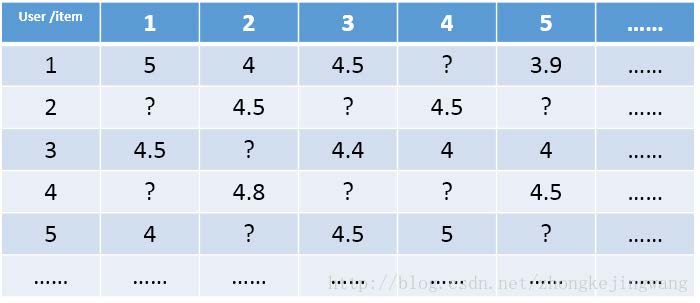
\includegraphics[width=7cm]{uesr_item.jpg}}
\caption{user-item matrix}
\end{figure}

Collaborative Filtering Algorithm has two types. The first one is memory-based. It uses user rating data to compute the similarity between users or items. Typical examples of this type are neighbourhood-based CF and item-based/user-based top-N recommendations. 
\begin{figure}[h]
\centerline{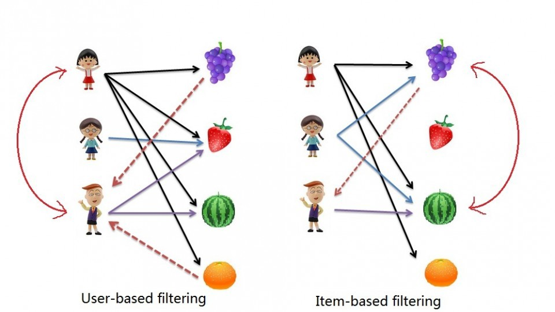
\includegraphics[width=7cm]{user_and_item.png}}
\caption{users' interest}
\end{figure}

For example, in user based types, the value of ratings user u gives to item i is calculated as an aggregation of some similar users' rating of the item:
\begin{equation}
r_{u,i}=aggr_{u'\in U}r_{u',i}
\end{equation}
where U denotes the set of top N users that are most similar to user u who rated item i. Some examples of the aggregation function includes:
\begin{equation}
r_{u,i}=\frac{1}{N}\sum_{u'\in U} r_{u',i}
\end{equation}
\begin{equation}
r_{u,i}=k\sum_{u'\in U}simil(u,u') r_{u',i}
\end{equation}
where k is a normalizing factor defined as
\begin{equation}
k=1/\sum_{u'\in U}|simil(u,u')|
\end{equation}
\begin{equation}
r_{u,i}=\bar{r_u}+k\sum_{u'\in U}(simil(u,u'))(r_{u',i}-\bar{r_{u'}})
\end{equation}
where $\bar{r_{u}}$ is the average rating of user u for all the items rated by u.

The neighborhood-based algorithm calculates the similarity between two users or items, and produces a prediction for the user by taking the weighted average of all the ratings. Similarity computation between items or users is an important part of this approach. Multiple measures, such as Pearson correlation and vector cosine based similarity are used for this.

The Pearson correlation similarity of two users x, y is defined as
\begin{equation}
simil (x,y)={\frac {\sum \limits _{i\in I_{xy}}(r_{x,i}-{\bar {r_{x}}})(r_{y,i}-{\bar {r_{y}}})}{{\sqrt {\sum \limits _{i\in I_{xy}}(r_{x,i}-{\bar {r_{x}}})^{2}}}{\sqrt {\sum \limits _{i\in I_{xy}}(r_{y,i}-{\bar {r_{y}}})^{2}}}}}
\end{equation}

where Ixy is the set of items rated by both user x and user y.

The cosine-based approach defines the cosine-similarity between two users x and y as\cite{breese1998empirical}:
\begin{equation}
simil (x,y)=\cos({\vec {x}},{\vec {y}})={\frac {{\vec {x}}\cdot {\vec {y}}}{||{\vec {x}}||\times ||{\vec {y}}||}}={\frac {\sum \limits _{i\in I_{xy}}r_{x,i}r_{y,i}}{{\sqrt {\sum \limits _{i\in I_{x}}r_{x,i}^{2}}}{\sqrt {\sum \limits _{i\in I_{y}}r_{y,i}^{2}}}}}
\end{equation}
The user-based top-N recommender algorithm uses a similarity-based vector model to identify the k users most similar to the active user. After finding the k most similar users, the corresponding user item matrices are aggregated to determine the set of items to recommend. A common method of finding similar users is location-sensitive hashing, which implements the nearest neighbor mechanism in linear time.

There are also several disadvantages with this type. Its performance decreases when data gets sparse, which occurs frequently with web-related items. This hinders the scalability of this type and creates problems with large datasets. Although it can efficiently handle new users because it relies on a data structure, adding new items becomes more complicated since that representation usually relies on a specific vector space. Adding new items requires inclusion of the new item and the re-insertion of all the elements in the structure.

The second type is Model-based\cite{Su:2009:SCF:1592474.1722966}. Models are developed using different data mining, machine learning algorithms to predict users' rating of unrated items. There are many model-based CF algorithms. Bayesian networks, clustering models, latent semantic models such as singular value decomposition, probabilistic latent semantic analysis, multiple multiplicative factor, latent Dirichlet allocation and Markov decision process based models\cite{su2009survey}. A potential way to get the user-item matrices is singular value decomposition. And our group is going to optimize the approach to get the SVD matrix\cite{takacs2009scalable}. $X = UDV^T$ ,where $U$ is an $m*m$ real matrix, D is an $m* n$ rectangular diagonal matrix with non-negative real numbers on the diagonal, and $V$ is an $n*n$ real matrix.

This paper mainly implement the basic Collaborative Filtering Algorithm, and based on it, we also implement the traditional SVD matrix factorization. Further on, our group proposed neural network based SVD\cite{he2017neural}.

\section{Background}
Appear and popularity of the Internet has brought a lot of information to users, and satisfy their demand of information in the information age. However, with the rapid development of network and the surge of online information, users may not be able to get the part which is really useful for themselves, and the efficiency of information reduce instead. This is also called information overload. 

Traditional information retrieval methods include classified catalog and search engine, which can solve the problem of information overload in some cases. Take the search engine as an example, its basic idea is similar to the classification contents, which is a used for sorting out the web pages and the information on the internet, but they use different technology. From the perspective of the process, the search engine first obtains the network information, and then sorts out, integrates and builds the index of the information. By querying inverted index, according to the content of the index and certain rules to calculate the relevance of user query content and web page, the search engine sorts and presents the web page to the user according to the relevance degree. Users can use keywords to find information which they are interested in, but when they cannot find keywords that accurately describe their needs, the search engine cannot achieve the search, which is also its limitations.

A very potential way to solve the problem of information overload is Recommender Systems, which is a personalized information Recommender System that recommends information and products to users according to their demands and interests. Compared with search engines, Recommender Systems conduct personalized calculation by studying users' preferences, and discover their interest by the system itself. Besides, the recommendation system can guide users to find their own information needs.A good recommender system can not only provide personalized services for users, but also establishes a close relationship with users, so that make users rely on recommendations. 

Obtaining recommendations from trusted sources is a critical component of the natural process of human decision making. With burgeoning consumerism buoyed by the emergence of the web, consumers are being presented with an increasing range of choices while sellers are being faced with the challenge of personalizing their advertising efforts. In parallel, it has become common for enterprises to collect large volumes of transactional data that allows for deeper analysis of how a customer base interacts with the space of product offerings. Recommender systems have evolved to full the natural dual need of buyers and sellers by automating the generation of recommendations based on data analysis.

\section{Motivation}
The user-item rating matrix is a sparse matrix, and for traditional singular value decomposition, the matrix should be dense, so that the algorithm needs to fill in vacancy by some ways, and the efficiency of singular value decomposition is still low. To solve these problem, we hope to optimize the SVD algorithm.
\section{RELATED WORK IN RECOMMENDATION ALGORITHM}
 The most widely used algorithm is collaborative filtering algorithm in recommendation system. Collaborative filtering methods are based on collecting and analyzing a large amount of information on users’ behaviors, activities or preferences and predicting what users will like based on their similarity to other users. A key advantage of the collaborative filtering approach is that it does not rely on machine analyzable content and therefore it is capable of accurately recommending complex items such as movies without requiring an "understanding" of the item itself. Collaborative filtering is based on the assumption that people who agreed in the past will agree in the future, and that they will like similar kinds of items as they liked in the past.In recent year, there are a lot of people use different way to improve recommend system's ability based on CF algorithm.such as traditional matrix factorization,k-nearest neighbor(k-NN) approach. there also have some people use deep learning  for recommendation.we think current methods although had got a good result, but algorithm time complexity and space complex is extremely high, it will cause bad results for for huge amount of  data.

\section{PROPOSED METHOD}
Based on the traditional SVD matrix factorization, we proposed neural network based SVD. since traditional SVD method has high time complexity and lower accuracy, so we pay more attention on those aspects of algorithm.
the traditional; SVD can decompose a matrix into three matrices use following equation:
\begin{equation}
X=UDV^T
\end{equation}
\begin{figure}[htbp]
	\centering
	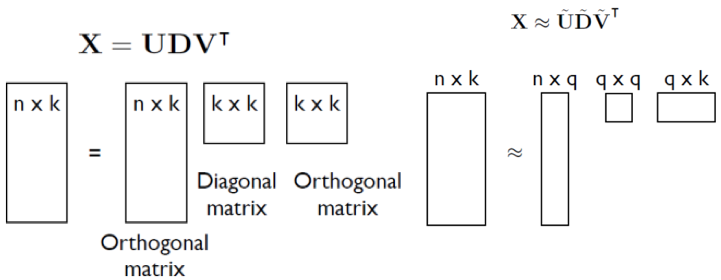
\includegraphics[width=0.7 \linewidth]{pa1}
	\caption{Traditional SVD}
	\label{fig:pa1}
\end{figure}
$U$ and $V^T$ are orthogonal matrices and $D$ is Diagonal matrix,since the elements of Diagonal matrix are eigenvalue of matrix and lower presentation eigenvalue include most feature of matrix. so we can choose $q<<k$ to reduce dimension of rating matrix and acculturate the speed of  recommendation.
\\
\subsection{First proposal: Neural based SVD}
using traditional way to do matrix factorization is slow and needs big space to save the matrix.For neural based SVD,we proposed that decompose rating matrix into two-dimensional matrices:
\begin{equation}
	R'=P^TQ,P\in R'^{f\cdot m},Q \in R'^{f\cdot n}
\end{equation} 
then we can find that the inner product of row vector of $P$ and column vector of $Q$ is the evaluation of user u to item i:
\begin{equation}
	R(i,j)=\sum_fp_{uf}q_{tf}
\end{equation}
how can we get matrices $P$ and  $Q$ from rating matrix $R'$?we use neural network to train training data and get result.assume  that known rating is $r_{ui}$,then the error between the true value and the predicted value is $e_{ui}=r_{ui}-\hat r_{ui}$.then we can use SSE as loss function and use Gradient descent method to train data.\\
by doing experiment we found that we got bad result by using this loss function to train data. the reason is overfitting,so we joined two regularization into our cost function and get new loss function:
\begin{equation}
\begin{aligned}
	SSE=&\sum_{u,i}e_{ui}^2+\frac{1}{2}\lambda \sum_u|p_u|^2+\frac{1}{2}\lambda \sum_i|q_i|^2\\
	=&\frac{1}{2}\sum_{u,i}e_{ui}^2+\frac{1}{2}\lambda \sum_{u}\sum_{k=0}^Kp^2_{uk}+\frac{1}{2}\lambda \sum_i\sum_{k=0}^Kq_{ki}^2
\end{aligned}
\end{equation}
then we use gradient descent to get updated value:($\alpha$ is learing rate)
\begin{equation}
\begin{split}
	p_{uk}:=p_{uk}+\alpha (e_{ui}q_{ki}-\lambda p_{uk})\\
	q_{ki}:=q_{ki}+\alpha (e_{ui}q_{uk}-\lambda p_{ik})
\end{split}
\end{equation}
\section{Second proposal:improved neural colloraborative filtering}
This proposal goes beyond our original expectations, we found a generalization neural network based framework for recommend system using collaboriative filtering algorithm.so we reimplemented original paper and proposed some ideal to improve this frames accuracy.\\
in this paper,the user used implicit data to represent rating,they define the user-item interaction matrix $Y\in R^{M\cdot N}$ as :
\begin{equation}
y_{ui}=\left\{
\begin{aligned}
1, & \text{if interaction (user u,item i) is observed;}\\
0, & \text{otherwise}
\end{aligned}
\right.
\end{equation}
Here a value of 1 for $y_{ui}$ indicates that there is an interaction between user u and item i; however, it does not mean u actually likes i. Similarly, a value of 0 does not necessarily mean u does not like i, it can be that the user is not aware of the item. \\
we think use $0-1$ to replace the original rating matrix is not accuray, it will lost a lot of information, so we use complete rating matrix as input and use the same framework to get the result.the author found that traditional SVD has some limitation, also including our proposal method has the same problem.\\
\begin{figure}[htbp]
	\centering
	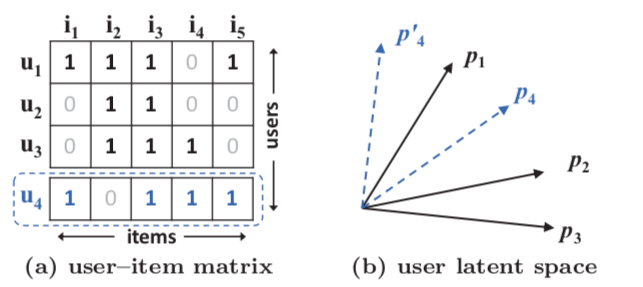
\includegraphics[width=7cm]{pa2}
	\caption{The limitation of Traditional SVD}
	\label{fig:pa2}
\end{figure}

Let us first focus on the first three rows (users) in Figure 2.by calculating cosine similarity between user 1,2 and 3. $s_{23}(0.82)>s_{12}(0.71)>s_{13}(0.58)$,when we add a user 4, we can find $s_{41}(0.75)>s_{43}(0.58)>s_{42}(0.35)$.but we can't place the $p_4$ properly in $b$. \\
so the author presented teh general neural collaborative filtering(NCF) framework. they adopt a multi-layer representation to model a user-item interaction $y_{ui}$,where the output of one layer serves as the input of the next one. the botton input layer consists of two feature vectors $v_u^U$ and $vi^I$ that describe user $u$ and item $i$,respectively;they can be customized to support a wide range of modelling of users and items,such as context-aware,content-based,and neighborbased.\\

\begin{figure}[htbp]
	\centering
	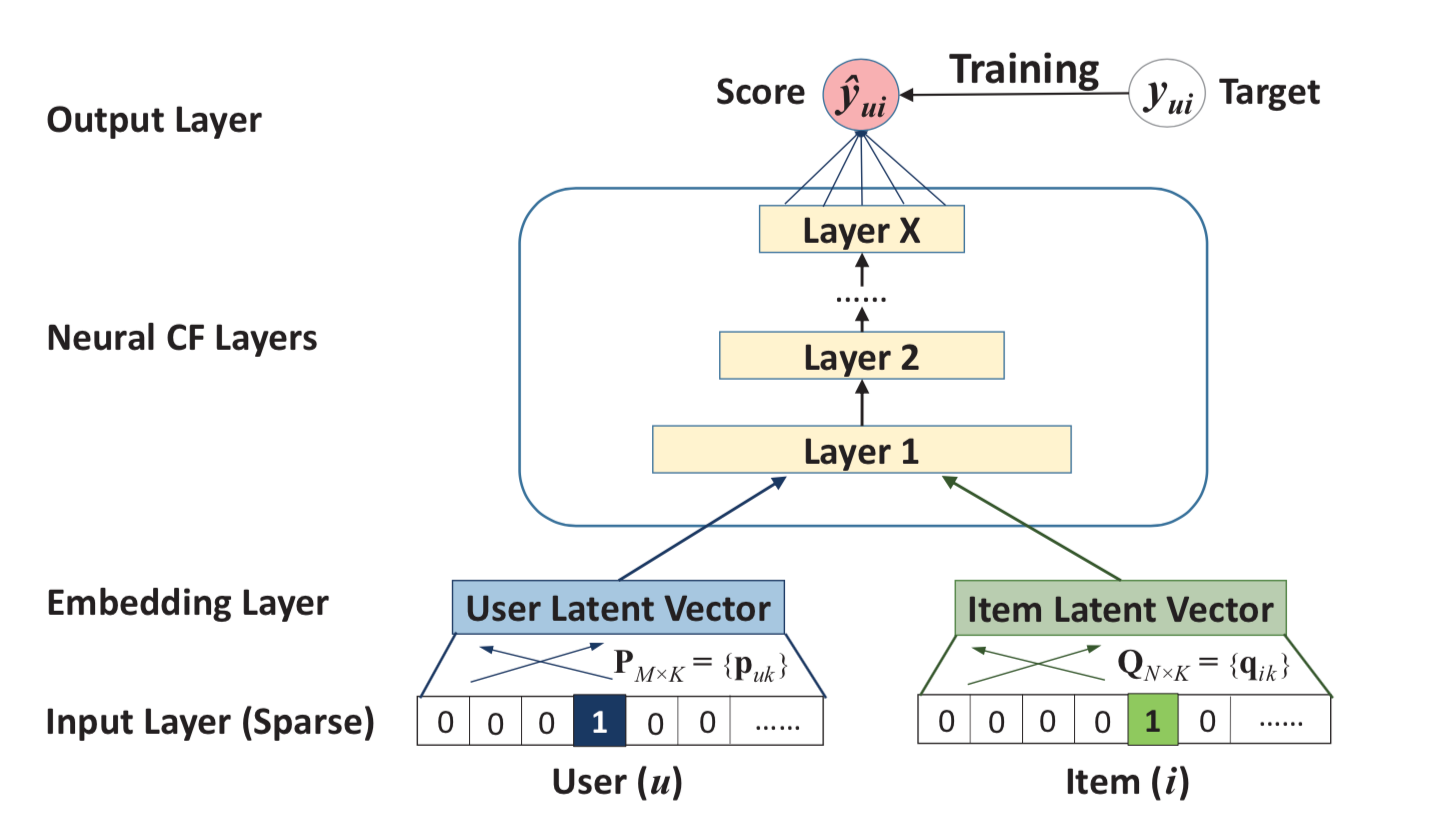
\includegraphics[width=7cm]{pa3}
	\caption{Neural collaborative filtering framework}
	\label{fig:pa3}
\end{figure}

Above the input layer is the embedding layer; it is a fully connected layer that projects the sparse representation to a dense vector. The obtained user (item) embedding can be seen as the latent vector for user (item) in the context of latent factor model. The user embedding and item embedding are then fed into a multi-layer neural architecture, which they term as neural collaborative filtering layers, to map the latent vectors to prediction scores. Each layer of the neural CF layers can be customized to discover certain latent structures of user-item interactions. The dimension of the last hidden layer $X$ determines the model’s capability. The final output layer is the predicted score $y_{ui}$, and training is performed by minimizing the pointwise loss between $y_{ui}$ and its target value $y_{ui}$. under this framework, they proposed three model.

\subsubsection{Generalized Matrix Factorization(GMF)}
this model is our proposed model's generalization, since in general framework they use one-hot encoding of user(item) ID of the input layer, the obtained embedding vector can be seen as the latent vector of user (item).Let the user latent vector $p_u$ be $P^T v^U_u$ and item latent vector qi be $Q^T v^I_i$ . We define the mapping function of the first neural CF layer as
\begin{equation}
	\phi_1(p_u,q_i)=p_u\odot q_i
\end{equation}
where $\odot$ denotes the element-wise product of vectors. then we can get the output layer is:
\begin{equation}
	\hat y_{ui}=\alpha_{out}(h^T(p_u\odot q_i))
\end{equation}
where $\alpha_{out}$ and $h$ denote the activation function and edge weights of the output layer, respectively. Intuitively, if we use an identity function for $\alpha_{out}$ and enforce $h$ to be a uniform vector of 1, we can the model which we have proposed.
\subsubsection{Multi-Layer Perceptron (MLP)}
the author use standard MLP to learn the interaction between user and item latent features.In this sense, they provide  the model a large level of flexibility and non-linearity to learn the interactions between $p_u$ and $q_i$, rather than the way of GMF that uses only a fixed element-wise product on them. More precisely, the MLP model under our NCF framework is defined as
\begin{equation}
\begin{aligned}
z_1=&\phi_1(p_u,q_i),\\
\phi_2(z_1)=&\alpha_{2}(W_2^Tz_1+b_2),\\
\cdots\\
\phi _L(L_1)=&\alpha_{L}(W_L^T z_{L-1}+b_L),\\
\hat y_{ui}=&\sigma(h^T\phi_L(z_{L-1}))
\end{aligned}
\end{equation}

where $W_x$, $b_x$, and $a_x$ denote the weight matrix, bias vec- tor, and activation function for the x-th layer’s perceptron, respectively.
\subsubsection{Fusion of GMF and MLP}
the author present the third model based on GMF and MLP model.since GMF  applies a linear kernel to model the latent feature interactions, and MLP that uses a non-linear kernel to learn the interaction function from data. by constructing a fusion model, they can mutually reinforce each other to better model the complex user-item interactions.the figure 4 shows the model.

\begin{figure}
	\centering
	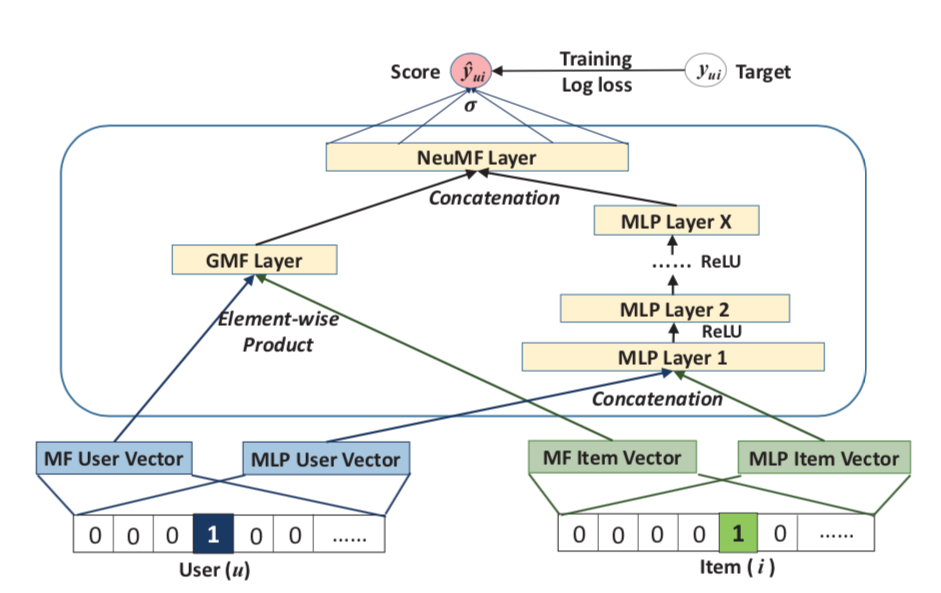
\includegraphics[width=7cm]{pa4}
	\caption{Fusion of GMF and MLP}
	\label{fig:pa4}
\end{figure}

A straightforward solution is to let GMF and MLP share the same embedding layer, and then combine the outputs of their interaction functions.This way shares a similar spirit with the well-known Neural Tensor Network(NTN).Specifically,the model for combining GMF with a one-layer MLP can be formulated as:
\begin{equation}
	\hat y_{ui}=\sigma(h^T a(p_u\odot q_i+W\cdot(p_u,q_i)+b))
\end{equation}
to provide more flexibility to the fused model,the author uses GMF and MLP to learn separate embeddings, and combone the two models by concatenating their last hidden layer.the formulation of which is given as follows:
\begin{equation}
\begin{aligned}
	\phi ^{GMF}=&p_u^G\odot q_i^G\\
	\phi ^{MLP}=&a_L(W_L^T(a_{L-1}(\cdots a_2(W_2^T\dot(p_u^M,q_i^M)+b_2)\cdots))+b_L)\\
	\hat y_{ui}=&\sigma(h^T(\phi^{GMP},\phi^{MLP}))
\end{aligned}
\end{equation}
where $p^G_u$ and $p^M_u$ denote the user embedding for GMF and MLP parts, respectively; and similar notations of $q^G_i$ and $q^M_i$ for item embeddings.
\section{Experiment}
\subsection{Implementation of Traditional CF and SVD}
in this project, we use the MovieLens 1M Dataset which is extremely famous in recommend system test.first let me give  brief introduction to this  dataset.this dataset includes 6040 users and 3704 items. so the rating matrix is $R^{6040\cdot 3704}$,which is huge.since each user usually make score to few movies,so the matrix is an extremely sparse matrix. our dataset's sparsity is:$95.6\%$.
\begin{figure}[h!]
	\centering
	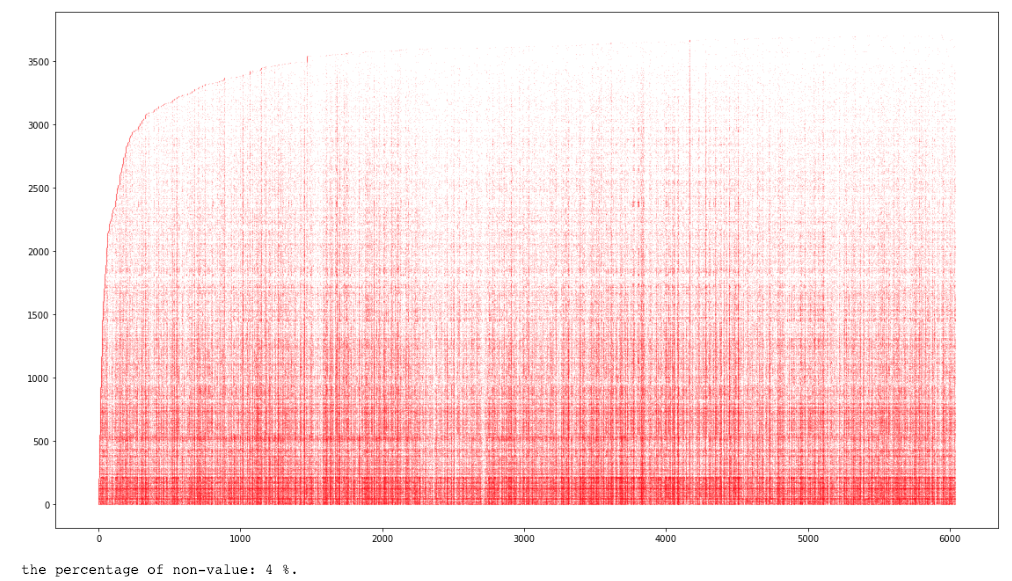
\includegraphics[width=7cm]{pa6}
	\caption{The  sparsity level of ml-1m dataset}
	\label{fig:pa6}
\end{figure}


for traditional CF,we use cosine similarity as similarity function:
\begin{equation}
	s_u^{cos}(u_k,u_a)=\frac{u_k\cdot u_a}{||u_k||||u_a||}=\frac{\sum x_{k,m}x_{a,m}}{\sqrt{\sum x_{k,m}^2}\sqrt{\sum x_{a,m}^2}}
\end{equation}

then the prediction function is:
\begin{equation}
	\bar x_{k,m}=\bar x_k+\frac{\sum_{u_a}(u_k,u_a)(x_{a,m}-\bar x_{u_a})}{\sum |sim_a(u_k,u_a)|}
\end{equation}


and the evaluation function is:
\begin{equation}
	RMSE=\sqrt{\frac{1}{N}\sum (x_i-\bar x_i)^2}
\end{equation}

for SVD method, we first use scipy's sparse to save the data and then decompose matrix into three matrix,then rebuild the rating matrix by different dimension of diagonal matrix and evaluate the result.(code can be see in ipython file).the result  is as follows:
\begin{figure}[h!]
	\centering
	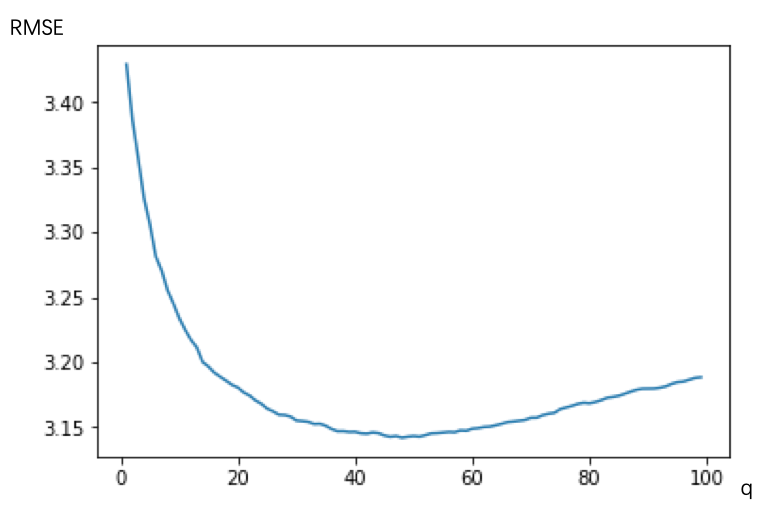
\includegraphics[width=7cm]{pa7}
	\caption{relationship between the number of diagonal matrix's element and RMSE}
	\label{fig:pa7}
\end{figure}

from this figure we can see that traditional SVD's accuracy is influenced by the number of diagonal matrix's element,the more number of elements , the higher accuracy we will get.
\begin{table}[h!]
	\centering
	\begin{tabular}{|l|l|}
		\hline
		{\ul \textbf{Method}} & {\ul \textbf{MSE}} \\ \hline
		User-based&3.35               \\ \hline
		Item-based&3.67                 \\ \hline
		SVD&3.14                 \\ \hline
	\end{tabular}
\end{table}
\subsubsection{Implementation of neural based SVD}
in this part, we use keras to implement the algorithm. in original state, the input is rating matrix $R$ and the output is $R'$.we use RMSE as our loss function and use adam as optimizer. we find that gradient descent very fast. in order to compare with that paper's result, we use hit rate as evaluation criteria.when we don't add regularization ,our highest hit rate is $60.24\%$;when we add two item as regularization, then best hit rate is $62.46\%$.we can find that add some regularization items have small improvement.
\subsubsection{Neural Collaborative Filtering}
for this part, we reimplemented that paper, this work had spend a lot of work.the dataset we still use ml-1m dataset, because we need to do compare with our own work result.in first step, we use a function to deal with data, if the entry of matrix is not equal to 0, then we changed it into 1,it's the way of author's paper.\\ For MLP model,we first input user(item) vector into a embedding layer,then through a flatten layer to change it into one dimension vector, and then concate the result,after this layer, we put the result into  MLP layers, which we used 8,16,32 and 64 layers.in order to get good result for non-linearity ability,we finally add a sigmoid function as activation function. for this model, we get best hit rate is $67.28\%$.\\

For GMF model, we did the same step to get user(item) vector, first input the data into embedding layers and then through a Flatten layers, in the next step we use element-wise product of user and item embeddings to get the result.from this step, we can find this model have few layers and extremely similarly to our model. we get best hit rate is $64.34\%$ for this model.\\

For fusion model, we first input the data into embedding layers and then through flatten layers.then we add MLP part and GMF part respectively, in final layer,we concatenate those to part and get the output.we found this model has a high ability to predict, its highest hit rate is  $68.69\%$.\\

when we changed input as real rate to replace the author's implicit data approach, we found have very small improvement, the hit rate is $70.21\%$,and we found if we use rate to do this work, we can't use some implicit information,including there exists interaction between user and items, but the user don't make score to items. so our proposed approach although have high hit rate for explicit  data, but lossing the ability to deal with the implicit data.so the author had considered more about implicit data and his model can be used more generalized.\\
by doing those work, we finally got the following result:
\begin{table}[h!]
	\centering
	\begin{tabular}{|l|l|}
		\hline
		{\ul \textbf{Method}} & {\ul \textbf{MSE}} \\ \hline
		SVD Based on Neural Network&62.46\%               \\ \hline
		GMF&64.34\%                \\ \hline
		MLP&67.28\%                 \\ \hline
		NeuMF&68.69\%                 \\ \hline
		NeuMF(improved)&70.21\%                 \\ \hline
	\end{tabular}
\end{table}

from this result, we found although our method result is lower then that paper's result, we still had done a big improvement compared with traditional SVD and CF algorithm. when we know that the author's general framework had  done a generalization of our approach and improved more, we had some disappointment,but we still learn from author and get a better result for explicit data,although this approach will completely lose the ability to model for implicit data. 


\section{Conclusion}
In this project, we implement the basic Collaborative Filtering Algorithm, and based on it, we also implement the traditional SVD matrix factorization. Besides, we also explored neural network SVD for collaborative filtering. We devised a general framework NCF and proposed three instantiations — GMF, MLP and NeuMF and get the result -- $NeuMF > MLP > GMF > SVD(Neural-based)>Traditional CF$


\appendix


% Bibliography
\bibliographystyle{ACM-Reference-Format-Journals}
\bibliography{reference}
                                % Sample .bib file with references that match those in
                                % the 'Specifications Document (V1.5)' as well containing
                                % 'legacy' bibs and bibs with 'alternate codings'.
                                % Gerry Murray - March 2012


\end{document}
% End of v2-acmtog-sample.tex (March 2012) - Gerry Murray, ACM
